
\subsection*{Overall Performance}

The unregularized neural network archetecture (N) was not a top performer for 
any of the six datasets. The other unregularized network, ordinary least 
squares (OLS) was the worst performer on every dataset. Ridge regression, 
a model with only L2 normalization, performed best on one dataset. 
LASSO regression, a form of L1 normalization that favors traits with few 
markers associated with moderate effects was not best on any dataset. 
Elastic Net is a regression technique that incorporates L2 and L1 
regularization together in a single model and was optimal on one dataset. 
Bayesian Ridge Regression incorporates L2 regularization, while also fitting 
regression coefficients to a gaussian distribution. It did not perform optimally 
on any problems, but frequenly performed above avreage. For the neural network family of 
regressors, at least one form of regularization outperformed the unregularized 
network for every dataset. Networks with both dropout and weight decay were 
able to achive best-in-dataset performance on two prediction tasks. These results are summarized 
in Table \ref{tab:model-comparison}.

These results support the hypothesis that some type of regularization is required to achieve
optimal performance in nerual network models. Additionally, a singular regularization strategy was
not optimal for all datasets, indicating that the best regularization strategy for genomic prediction
is dependent on the predicted species, trait, or population studied. 

Dropout regularization tends to produce networks 
that have reduced co-adaptation \citep{srivastava2014}. For genomic prediction tasks, this would
indicate that the detection of rare combinations haplotypes specific to only one
or two individuals are generally not learned or used for prediction. Instead, common haplotypes that persist across many
different dropout iterations would be preferred and associated with phenotypic performance by the network during training.

Weight decay is an application of L2 regularization to neural networks \citep{krogh1992}. Like ridge regression, it prefers
solutions that do not place large emphasis on any singular feature. For genomic prediction tasks, 
this will produce models that perform well on traits with many predictive marker calls 
with small effects. 

For traits with a mixture of a few large-effect alleles and many small effect allels, some combination of 
L1 and L2 regularization may be optimal. The elastic net (EN) model incorporates both of these regularization
techniques, and is the top performer on two of the six datasets presented.

Several models with notably high performance that were not included in this analysis include a
family of bayesian regression models known as the "bayesian alphabet" \citep{gianola2009}. These
models apply regularization by assuming prior distributions over the number of contributing markers
and the magnitude of their effects on a realized phenotype. Another category of model, Reproducing 
Kernel Hilbert Spaces (RKHS) regression has shown promise on a wide variety of genomic 
prediction tasks \citep{heslot2012, gianola2008}. Regularization in RKHS regression is achieved
by favoring predictive functions with "smooth" functional forms. Standard implementations
of the bayesian family of regressors as well as RKHS models were not included in this analysis
because they do not yet have standard implementations in the python computing libraries used 
to conducted the experiment presented in this article.

\ifdefined\showtablesandfigures
% Benchmark Datasets table.

\begin{table*}[htbp]
    \renewcommand{\familydefault}{\sfdefault}\normalfont
    \centering
    \caption{\bf Model Performance}

    \begin{tableminipage}{\textwidth}

        \begin{tabularx}{\textwidth}{ m{4.8em} m{4.8em} m{1.6em} m{1.6em} m{2.2em} m{1.6em} m{1.6em} m{1.6em} m{1.6em} m{1.6em} m{2.2em} }
\hline
\header & & \multicolumn{9}{c}{Accuracy} \\
\header & & OLS & RR & LASSO & EN & BRR & N & NWD & NDO & NWDDO \\
\hline
\header Species & Trait & & & & & & & & & \\
\hline
Arabidopsis & Dry Matter & 0.36 & 0.40 & 0.40 & \underline{0.42} & 0.39 & 0.38 & 0.35 & 0.39 & 0.40 \\
  & Flowering & 0.80 & 0.82 & 0.83 & 0.82 & 0.82 & 0.84 & 0.83 & 0.83 & \underline{0.86} \\
\hline
Maize & Flowering & 0.22 & 0.33 & 0.32 & 0.33 & 0.32 & 0.33 & 0.34 & \underline{0.35} & 0.33 \\
  & Grain Yield & 0.47 & \underline{0.59} & 0.49 & 0.51 & 0.57 & 0.55 & 0.52 & 0.55 & 0.51 \\
\hline
Wheat & Spike Grain Number & 0.15 & 0.27 & 0.33 & \underline{0.36} & 0.28 & 0.27 & 0.31 & 0.28 & 0.33 \\
  & Time Young Microspore & 0.59 & 0.61 & 0.74 & 0.73 & 0.64 & 0.67 & 0.74 & 0.68 & \underline{0.76} \\
\hline
\end{tabularx}

        \label{tab:model-comparison}
        \footnotesize  

        Accuracy of the best observed model performance on each dataset,
        rounded to three decimal places. The most accurate model on 
        each dataset is underlined for emphasis. 
        
    \end{tableminipage}
\end{table*}
 % Label = tab:model-comparison
\fi

\subsection*{Regularized Network Performance}

If a model is overfitted to training data, training data prediction accuracy is greater than 
the accuracy observed when making predictions on new datasets. Regularization methods
generally penalize models for overfitting to data. Because all measurements in this study 
were collected using five-fold cross validation sampling, models that exhibited overfitting 
should exhibit lower accuracy. 

The decreased performance of the unregularized networks on several datasets in Figure 
\ref{fig:network-comparison} suggests that overfitting is sometimes, but not always
a problem with genomic prediction applications. These results demonstrate that 
evaluating one or more regularization methods is critical to improve predictive accuracy for 
genomic prediction.

\ifdefined\showtablesandfigures

\begin{figure}[htbp]
\renewcommand{\familydefault}{\sfdefault}\normalfont
\centering 
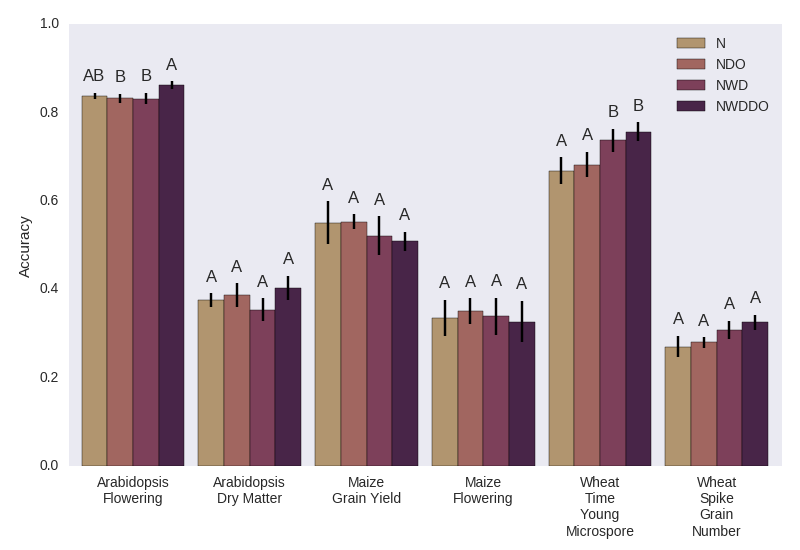
\includegraphics[width=\linewidth]{g3_article/figures/network_comparison.png}
    \caption{Predictive accuracy ($\mu \pm \sigma_{\bar{x}}$) of 
             regularized and non-regularized 
             neural network models for on benchmark datasets. Only the best performing
             network archetecture for each species, trait, and model is included. 
             The accuracy of the best performing model across all folds of data 
             and training cycles were recorded and compared. All pairwise model 
             comparisons within a species and trait were made using a two-sided paired t-test 
             (n=10, paired by training cycle and fold number).
             The resulting p-values were corrected for multiple comparisons within each 
             species and trait combination using the Holm-Bonferroni method. Columns annotated 
             with the same letter are not significantly different 
             at the $\alpha=0.05$ level.}
\label{fig:network-comparison}
\end{figure}
 % Label = fig:network-comparison
\fi

\subsection*{Deep Network Performance}

Contrary to expectation, neural networks with additional hidden layers did not perform
significantly better than networks with a single layer (Figure \ref{fig:depth-comparison}). 
One possible explanation for this observation is that by the universal approximation theorem,
sufficiently large single layer neural networks can approximate any function, including those
that deeper networks can approximate. In this study, single layer networks up to and including
those with 2187 ($3^7$) neurons were evaluated on all datasets. This number is larger than the number
of markers in any dataset evaluated and may be enough to encode complex interactions in only a single
layer.

Networks with deep archetectures have proven effective on a wide variety of problems, but the largest
improvents have occurred on problems with high dimensional input data. These include voice recognition 
tasks where vocal frequencies change over a time dimension or two-dimensional images change over 
a time dimension such as in video playback. It is possible that the dimensionality of genomic 
prediction tasks presented in this article are insufficient to benefit from the deep interaction 
effects that have proven effective in prediction tasks in other domains. 

Yet another possibility is that phenotypic measurement error on many datasets is large enough 
to mask the subtle interaction effects that would otherwise be learned by the network.

\ifdefined\showtablesandfigures

\begin{figure}[htbp]
\renewcommand{\familydefault}{\sfdefault}\normalfont
\centering 
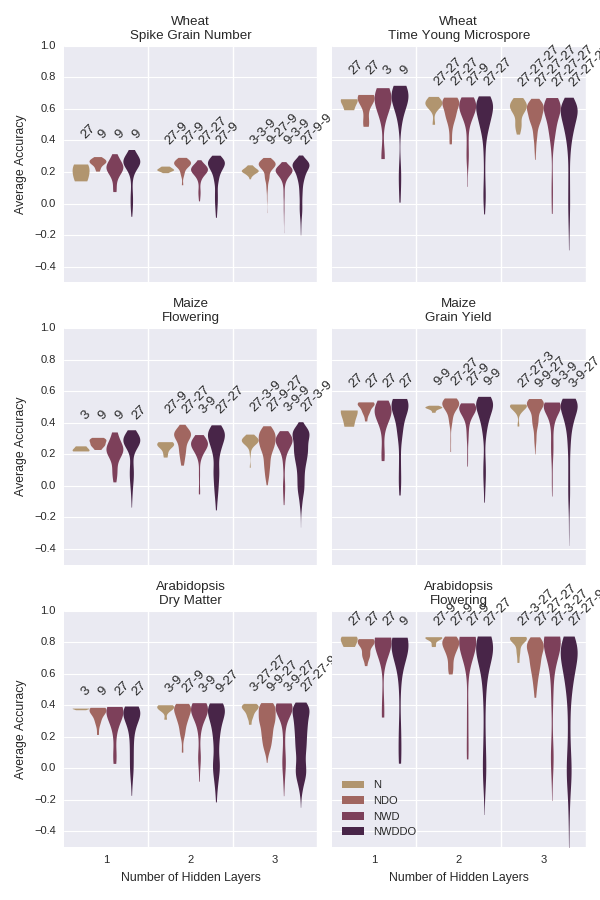
\includegraphics[keepaspectratio,height=\textheight,width=\linewidth]{g3_article/figures/depth_comparison.png}
    \caption{Distribution of predictive accuracy by benchmark dataset, network depth, 
             and model. The violin plot width indicates the Kernel Density Estimate 
             (KDE) of all observed accuracies of all models at a given network depth. 
             The sample size of the KDE is 7, 28, 28, and 112 samples for the 
             N, NWD, NDO, and NWDDO models, respectively. The models contributing 
             to each KDE vary across one or more of five weight decay, five dropout, 
             and seven hidden layer architecture parameters and can be 
             understood as the distribution of results across the set of 
             hyper-parameters to all network models with the same depth and regularization
             type. The KDE bandwidth parameters are set using Scott's normal reference rule. 
             The KDE plots are truncated to the minimum and maximum observed prediction accuracies.} 
\label{fig:depth-comparison}
\end{figure}

 % Label = fig:depth-comparison
\fi

\subsection*{GPU and CPU Training Time}

Network training time was significantly different from CPU training time in all datasets 
(Figure \ref{fig:time-comparison}).  For small networks trained on smaller datasets 
such as arabidopsis, CPU training completed significantly faster than GPU training, 
though only by a small magnitude. For small networks and all other datasets, as well 
as for all large networks, GPU training time was faster than CPU training time on a 
per-core basis. These results confirm that the speedups associated 
with GPU network training apply to genomic selection applications.  


%For very large datasets such as the pig and loblolly datasets, CPU 
%computing could not be completed in under 24 hours, but could be completed by a 
%dedicated GPU card during that time. 

The results from Figure \ref{fig:time-comparison} compare a single Intel i7-4790K CPU 
core to a single Nvidia GTX 680 graphics card. However, most modern full-size computers posess 
multiple CPU cores, but few contain graphics cards with GPU compute capability. 
Thus, choosing a network training method depends on computing hardware availability 
as well as required turnaround time. Cloud providers such as Amazon Web Services (AWS) 
are becoming more popular, and make this choice somewhat less important. AWS 
provides both CPU and GPU rich machines which can be rented at low cost and 
are charged by the hour. This makes it feasible to choose a training platform 
that is most cost effective based on the quantity of data and desired network 
archetecture for any genomic selection application.

\ifdefined\showtablesandfigures

\begin{figure}[htbp]
\renewcommand{\familydefault}{\sfdefault}\normalfont
\centering 
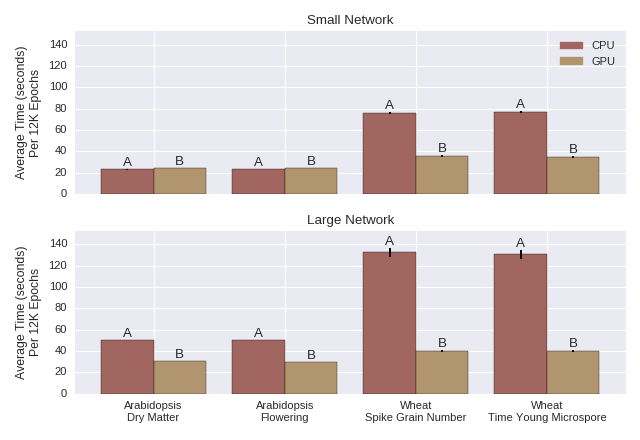
\includegraphics[keepaspectratio,width=\linewidth,height=\textheight]{g3_article/figures/time_comparison.png}
    \caption{Time to train different sized networks on identical datsets using a single dedicated CPU core
             compared to a single dedicated GPU card. Lower time to train is better. For the small network, 
             an unregularized, single hidden layer of 27 neurons was trained for 12K epochs on each dataset. 
             For the large network, two the hidden layers of size 64 and 32 neurons, respectively were trained. 
             Training processes were otherwise equal. This process was repeated ten times per dataset to 
             reduce variation associated with non-deterministic processor scheduling and varying computer system load.
             The ten CPU and GPU training samples were compared using an independent samples T-test with $n=30$. 
             CPU-GPU pairs annotated with the same letter are not significantly different 
             at the $\alpha=0.05$ level.}
\label{fig:time-comparison}
\end{figure}
 % Label = fig:time-comparison
\fi

\subsection*{Overall Conclusion}

When combined with effective regularization techniques, neural networks can function
as accurate and effective genomic prediction models with a low risk of overfitting
to training data. When trained with GPU computation resources, concerns
over total time to train are partially ameliorated. Searches for optimal archetectures or 
regularization techniques can be automated in a time and cost effective 
manner using cloud compute providers such as AWS.

While algorithms such as RKHS regression and neural networks sometimes produce
genomic prediction models with high predictive accuracy. Models such as these
capture interaction effects between groups of one or more markers and thus 
predict phenotypes rather than GBLUPs. As a result, caution must be exercised when interpreting 
improved prediction accuracy as a better model in the general case. Applications 
to breeding scenarios where additive genetic gain is of lesser importance 
may prove more effective. Examples include breeding clonal crop varieties or 
making optimal breeding crosses that maximize the likelihood of producing
transgressive segregates.
